\def\backupslinklabel#1{\label{backups-#1}}
\def\backupslinkref#1#2{\submanip #2~\hyperlink{backups-#1}{\beamerskipbutton{slide~\ref{backups-#1}}}}

\begin{frame}[label=backups]

\manip Phenomenology:
\backupslinkref{pheno}{SM, SUSY, 2HDM, $\tan\beta$}
\backupslinkref{histos}{How histograms unveil particles}

\manip JERC with \Gjets\ events:
\backupslinkref{JEC}{Jet energy calibration}
\backupslinkref{JER}{Jet energy resolution}

\manip MSSM \HAtoTauTau:
\backupslinkref{trgeffs}{Triggers in the \tauh\tauh\ channel}
\backupslinkref{subleadingFtauh}{\Fakefactors\ for subleading \tauh}

\manip Machine Learning:
\backupslinkref{custom_loss}{Custom loss function for the DNN}

\end{frame}

\subsection*{The standard model}
\begin{frame}
\frametitle{The Standard Model}
\begin{center}
\ifdefined\homedir \else \def\homedir{/home/torterotot}\fi
\IfFileExists{\homedir/Dropbox/Enseignement/TikZ_files/modele_standard_EN/init.tex}{
\includegraphics[scale=.575]{\PhDthesisdir/tex/slides/SM_MSSM_HTT_pheno/SM_and_its_limits/_SM2018.tex}
}{
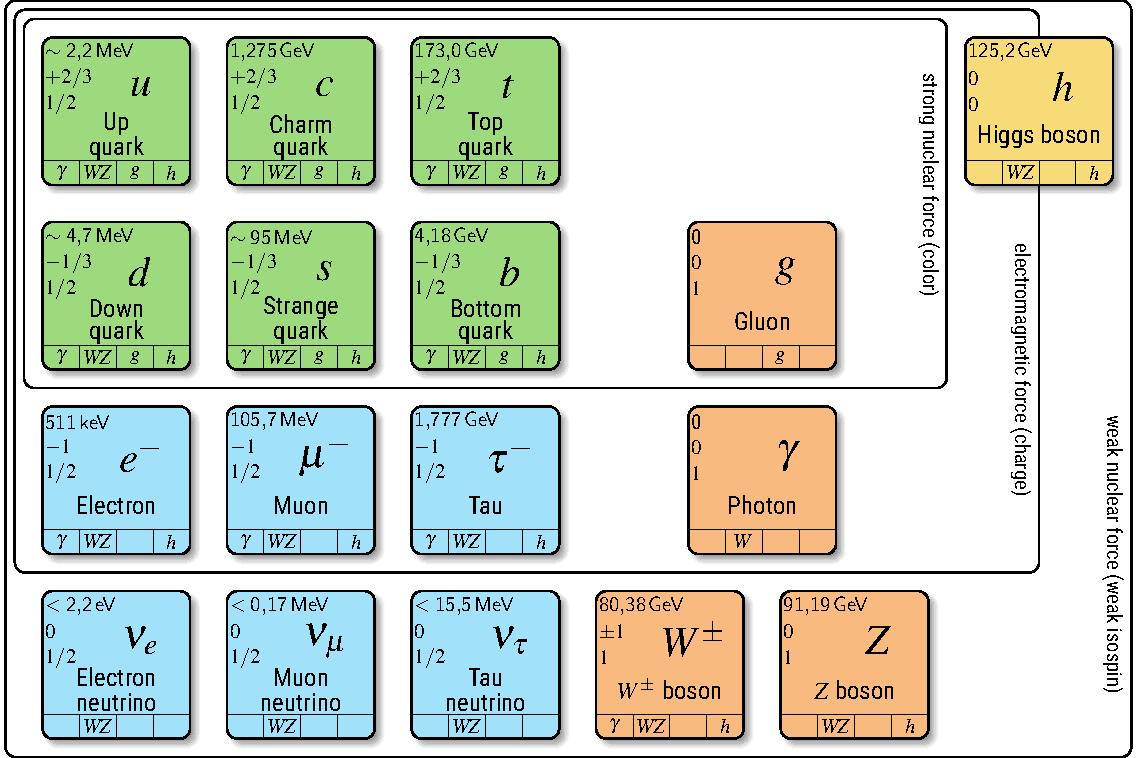
\includegraphics[scale=.575]{\PhDthesisdir/tex/slides/SM_MSSM_HTT_pheno/SM_and_its_limits/SM_2018-bak.pdf}
}
\end{center}
\end{frame}

\begin{frame}
\frametitle{The Standard Model and naturalness problem}

\manip Higgs mass measured: $m_{\higgs} = \num{125.10} \pm \SI{0.14}{\GeV}$\beamercite{PDG_booklet_2020}

\manip Higgs mass derivation:
$\displaystyle
m_{\higgs}^2 = m_{\higgs 0}^2 -\frac{3}{8\pi^2} y_{\quarkt}^2 \Lambda^2  +\frac{1}{16\pi^2} g^2 \Lambda^2 + \frac{1}{16\pi^2} \lambda^2 \Lambda^2 + \ldots
$

\begin{minipage}[t]{.3\textwidth}
\begin{block}{top quark}
\begin{center}
\vspace{-4.5pt}
\begin{fmffile}{Higgs_loop_fermion}\fmfstraight
\begin{fmfchar*}(30,20)
  \fmfleft{i}
  \fmfright{o}
  \fmf{dashes}{i,v1}
  \fmf{dashes}{v2,o}
  \fmf{fermion,left,tension=.3}{v1,v2,v1}
  \fmfdot{v1,v2}
  \fmflabel{ }{i}
\end{fmfchar*}
\end{fmffile}

\vspace{-4.5pt}

$\displaystyle -\frac{3}{8\pi^2} y_{\quarkt}^2 \Lambda^2 \sim -(\SI{2}{\TeV})^2$
\end{center}
\end{block}
\end{minipage}
\hfill
\begin{minipage}[t]{.3\textwidth}
\begin{block}{vector bosons}
\begin{center}
\begin{fmffile}{Higgs_loop_gauge}\fmfstraight
\begin{fmfchar*}(30,20)
  \fmfleftn{i}{4}
  \fmfrightn{o}{4}
  \fmf{dashes}{i2,v,o2}
  \fmf{phantom}{i4,vbis,o4}
  \fmffreeze
  \fmf{boson, right}{v,vbis,v}
  \fmfdot{v}
  \fmflabel{ }{i2}
\end{fmfchar*}
\end{fmffile}

\vspace{-9pt}

$\displaystyle +\frac{1}{16\pi^2} g^2 \Lambda^2 \sim +(\SI{0.7}{\TeV})^2$
\end{center}
\end{block}
\end{minipage}
\hfill
\begin{minipage}[t]{.3\textwidth}
\begin{block}{Higgs itself}
\begin{center}
\begin{fmffile}{Higgs_loop_sfermion}\fmfstraight
\begin{fmfchar*}(30,20)
  \fmfleftn{i}{4}
  \fmfrightn{o}{4}
  \fmf{dashes}{i2,v,o2}
  \fmf{phantom}{i4,vbis,o4}
  \fmffreeze
  \fmf{dashes, right}{v,vbis,v}
  \fmfdot{v}
  \fmflabel{ }{i2}
\end{fmfchar*}
\end{fmffile}

\vspace{-9pt}

$\displaystyle + \frac{1}{16\pi^2} \lambda^2 \Lambda^2 \sim +(\SI{0.5}{\TeV})^2$
\end{center}
\end{block}
\end{minipage}

\end{frame}

\begin{frame}
\frametitle{Supersymmetry}

\begin{minipage}[t]{.3\textwidth}
\begin{block}{top quark}
\begin{center}
\vspace{-4.5pt}
\begin{fmffile}{Higgs_loop_fermion}\fmfstraight
\begin{fmfchar*}(30,20)
  \fmfleft{i}
  \fmfright{o}
  \fmf{dashes}{i,v1}
  \fmf{dashes}{v2,o}
  \fmf{fermion,left,tension=.3}{v1,v2,v1}
  \fmfdot{v1,v2}
  \fmflabel{ }{i}
\end{fmfchar*}
\end{fmffile}

\vspace{-4.5pt}

$\sim -(\SI{2}{\TeV})^2$
\end{center}
\end{block}
\end{minipage}
\hfill
\begin{minipage}[t]{.3\textwidth}
\begin{block}{vector bosons}
\begin{center}
\begin{fmffile}{Higgs_loop_gauge}\fmfstraight
\begin{fmfchar*}(30,20)
  \fmfleftn{i}{4}
  \fmfrightn{o}{4}
  \fmf{dashes}{i2,v,o2}
  \fmf{phantom}{i4,vbis,o4}
  \fmffreeze
  \fmf{boson, right}{v,vbis,v}
  \fmfdot{v}
  \fmflabel{ }{i2}
\end{fmfchar*}
\end{fmffile}

\vspace{-9pt}

$\sim +(\SI{0.7}{\TeV})^2$
\end{center}
\end{block}
\end{minipage}
\hfill
\begin{minipage}[t]{.3\textwidth}
\begin{block}{Higgs itself}
\begin{center}
\begin{fmffile}{Higgs_loop_sfermion}\fmfstraight
\begin{fmfchar*}(30,20)
  \fmfleftn{i}{4}
  \fmfrightn{o}{4}
  \fmf{dashes}{i2,v,o2}
  \fmf{phantom}{i4,vbis,o4}
  \fmffreeze
  \fmf{dashes, right}{v,vbis,v}
  \fmfdot{v}
  \fmflabel{ }{i2}
\end{fmfchar*}
\end{fmffile}

\vspace{-9pt}

$\sim +(\SI{0.5}{\TeV})^2$
\end{center}
\end{block}
\end{minipage}


\begin{minipage}[t]{.3\textwidth}
\begin{block}{stop quark}
\begin{center}
\begin{fmffile}{Higgs_loop_sfermion}\fmfstraight
\begin{fmfchar*}(30,20)
  \fmfleftn{i}{4}
  \fmfrightn{o}{4}
  \fmf{dashes}{i2,v,o2}
  \fmf{phantom}{i4,vbis,o4}
  \fmffreeze
  \fmf{dashes, right}{v,vbis,v}
  \fmfdot{v}
  \fmflabel{ }{i2}
\end{fmfchar*}
\end{fmffile}

\vspace{-9pt}

$\sim +(\SI{2}{\TeV})^2$
\end{center}
\end{block}
\end{minipage}
\hfill
\begin{minipage}[t]{.3\textwidth}
\begin{block}{bosinos}
\begin{center}
\vspace{-4.5pt}
\begin{fmffile}{Higgs_loop_fermion}\fmfstraight
\begin{fmfchar*}(30,20)
  \fmfleft{i}
  \fmfright{o}
  \fmf{dashes}{i,v1}
  \fmf{dashes}{v2,o}
  \fmf{fermion,left,tension=.3}{v1,v2,v1}
  \fmfdot{v1,v2}
  \fmflabel{ }{i}
\end{fmfchar*}
\end{fmffile}

\vspace{-4.5pt}

$\sim -(\SI{0.7}{\TeV})^2$
\end{center}
\end{block}
\end{minipage}
\hfill
\begin{minipage}[t]{.3\textwidth}
\begin{block}{Higgsinos}
\begin{center}
\vspace{-4.5pt}
\begin{fmffile}{Higgs_loop_fermion}\fmfstraight
\begin{fmfchar*}(30,20)
  \fmfleft{i}
  \fmfright{o}
  \fmf{dashes}{i,v1}
  \fmf{dashes}{v2,o}
  \fmf{fermion,left,tension=.3}{v1,v2,v1}
  \fmfdot{v1,v2}
  \fmflabel{ }{i}
\end{fmfchar*}
\end{fmffile}

\vspace{-4.5pt}

$\sim -(\SI{0.5}{\TeV})^2$
\end{center}
\end{block}
\end{minipage}

\end{frame}

%\begin{frame}
%\frametitle{Naturalness and supersymmetry}
%\manip Higgs mass: $\displaystyle m_{\higgs}^{2}=2\mu ^{2}+\delta m_{\higgs}^{2} \simeq \SI{125}{\GeV}$
%\begin{equation*}
%\delta m_{\higgs}^{2}\simeq {\frac {3}{4\pi ^{2}}}{\Bigl (}-\lambda _{\quarkt}^{2}+{\frac {g^{2}}{4}}+{\frac {g^{2}}{8\cos ^{2}\theta _{W}}}+\lambda {\Bigr )}\Lambda ^{2}
%\end{equation*}
%
%For instance, if one includes see-saw neutrinos into the Standard Model, then $\delta m_{\higgs}$ would blow up to near the see-saw scale, typically expected in the \SI{e13}{\GeV} range. 
%
%\end{frame}
%
%\begin{frame}
%\frametitle{Naturalness and supersymmetry}
%\manip By supersymmetrizing the Standard Model, one arrives at a solution to the gauge hierarchy, or big hierarchy, problem in that supersymmetry guarantees cancellation of quadratic divergences to all orders in perturbation theory.
%
%\begin{fmffile}{Higgs_loop_fermion}\fmfstraight
\begin{fmfchar*}(30,20)
  \fmfleft{i}
  \fmfright{o}
  \fmf{dashes}{i,v1}
  \fmf{dashes}{v2,o}
  \fmf{fermion,left,tension=.3}{v1,v2,v1}
  \fmfdot{v1,v2}
  \fmflabel{ }{i}
\end{fmfchar*}
\end{fmffile}

%
%\begin{fmffile}{Higgs_loop_sfermion}\fmfstraight
\begin{fmfchar*}(30,20)
  \fmfleftn{i}{4}
  \fmfrightn{o}{4}
  \fmf{dashes}{i2,v,o2}
  \fmf{phantom}{i4,vbis,o4}
  \fmffreeze
  \fmf{dashes, right}{v,vbis,v}
  \fmfdot{v}
  \fmflabel{ }{i2}
\end{fmfchar*}
\end{fmffile}

%
%\end{frame}

\begin{frame}
\frametitle{2 Higgs doublets models for supersymmetry}
\begin{equation*}
\average{\phi_1}_0 = \frac{1}{\sqrt{2}} \begin{pmatrix}
0\\v_1
\end{pmatrix}
\msep
\average{\phi_2}_0 = \frac{1}{\sqrt{2}} \begin{pmatrix}
0\\v_2 \eexp{\im\xi}
\end{pmatrix}
\end{equation*}

\begin{equation*}
\boxed{\tan\beta = \frac{\average{\phi_2}_0}{\average{\phi_1}_0} = \frac{v_2}{v_1}}
\end{equation*}

\beamercite{Higgs_hunter_guide}
\end{frame}

\subsection*{Why histograms}
\begin{frame}
\frametitle{Using histograms}

\manip Find a discriminating variable:
\submanip for uncorrelated \tau\ pairs, it's random
\submanip for \tau\ pairs coming from a particle (Higgs?), not random.

\manip For one \tau\ pair only, impossible to say!

\manip With many events, a difference may show up.
\end{frame}

\begin{frame}
\frametitle{The rabbit analogy}
\beamercite{Higgs_discovery_explained_video_3}

\manip White rabbit that once lived in a casino.
\submanip The rabbit loved watching people playing dices.
\submanip He was happy when the result of dice was 4.
\submanip So when he sees a dice, he turns it so that the result is 4.
\submanip But this rabbit is very shy and nobody has seen him since the casino closure.
\submanip The only way to know if he's here is to throw a dice and come back to see the result.
\submanip If the rabbit has been here, the dice will show a 4!
\end{frame}

\begin{frame}
\frametitle{The rabbit analogy}
\beamercite{Higgs_discovery_explained_video_3}

\manip Dice results:
4\pause,
2\pause,
4,
1,
3,
2,
5,
1,
1,
6...
\end{frame}

\begin{frame}
\frametitle{The rabbit analogy}
\beamercite{Higgs_discovery_explained_video_3}
\begin{center}
\begin{minipage}[c]{.29\textwidth}
On \num{100} days $\rightarrow$
\end{minipage}
\begin{minipage}[c]{.4\textwidth}
\vspace{-\baselineskip}
\includegraphics[height=\graphh, width=\graphw,keepaspectratio]{/home/torterotot/Documents/PhD-Thesis/plots_and_images/my_plots/inspired_from_Higgs_discovery_explained_video_3/1-only_data_100-pyplot.tex}
\end{minipage}
\begin{minipage}[c]{.29\textwidth}
Not really conclusive...
\end{minipage}
\end{center}
\end{frame}

\begin{frame}
\frametitle{The rabbit analogy}
\addtocounter{framenumber}{-1}
\beamercite{Higgs_discovery_explained_video_3}
\begin{center}
\begin{minipage}[c]{.29\textwidth}
On \num{100} days $\rightarrow$
\end{minipage}
\begin{minipage}[c]{.4\textwidth}
\vspace{-\baselineskip}
\includegraphics[height=\graphh, width=\graphw,keepaspectratio]{/home/torterotot/Documents/PhD-Thesis/plots_and_images/my_plots/inspired_from_Higgs_discovery_explained_video_3/2-data_and_bg_estim_100-pyplot.tex}
\end{minipage}
\begin{minipage}[c]{.29\textwidth}
Comparing with predictions!
\end{minipage}
\end{center}
\end{frame}

\begin{frame}
\frametitle{The rabbit analogy}
\addtocounter{framenumber}{-1}
\beamercite{Higgs_discovery_explained_video_3}
\begin{center}
\begin{minipage}[c]{.29\textwidth}
On \num{100} days $\rightarrow$
\end{minipage}
\begin{minipage}[c]{.4\textwidth}
\vspace{-\baselineskip}
\includegraphics[height=\graphh, width=\graphw,keepaspectratio]{/home/torterotot/Documents/PhD-Thesis/plots_and_images/my_plots/inspired_from_Higgs_discovery_explained_video_3/3-data_and_bg_estim_ratio_100-pyplot.tex}
\end{minipage}
\begin{minipage}[c]{.29\textwidth}
Also add ratio plot:\\
observed / predictions
\end{minipage}
\end{center}
\end{frame}

\begin{frame}
\frametitle{The rabbit analogy}
\addtocounter{framenumber}{-1}
\beamercite{Higgs_discovery_explained_video_3}
\begin{center}
\begin{minipage}[c]{.29\textwidth}
On \num{100} days $\rightarrow$
\end{minipage}
\begin{minipage}[c]{.4\textwidth}
\vspace{-\baselineskip}
\includegraphics[height=\graphh, width=\graphw,keepaspectratio]{/home/torterotot/Documents/PhD-Thesis/plots_and_images/my_plots/inspired_from_Higgs_discovery_explained_video_3/4-up_to_100-pyplot.tex}
\end{minipage}
\begin{minipage}[c]{.29\textwidth}
Fill up with more data!
\end{minipage}
\end{center}
\end{frame}

%\begin{frame}
%\frametitle{The rabbit analogy}
%\addtocounter{framenumber}{-1}
%\transwipe[direction=90]
%\beamercite{Higgs_discovery_explained_video_3}
%\begin{center}
%\begin{minipage}[c]{.29\textwidth}
%On \num{500} days $\rightarrow$
%\end{minipage}
%\begin{minipage}[c]{.4\textwidth}
%\vspace{-\baselineskip}
%\includegraphics[height=\graphh, width=\graphw,keepaspectratio]{/home/torterotot/Documents/PhD-Thesis/plots_and_images/my_plots/inspired_from_Higgs_discovery_explained_video_3/5-up_to_500-pyplot.tex}
%\end{minipage}
%\begin{minipage}[c]{.29\textwidth}
%Fill up with more data!
%\end{minipage}
%\end{center}
%\end{frame}

\begin{frame}
\frametitle{The rabbit analogy}
\addtocounter{framenumber}{-1}
\transwipe[direction=90]
\beamercite{Higgs_discovery_explained_video_3}
\begin{center}
\begin{minipage}[c]{.29\textwidth}
On \num{1000} days $\rightarrow$
\end{minipage}
\begin{minipage}[c]{.4\textwidth}
\vspace{-\baselineskip}
\includegraphics[height=\graphh, width=\graphw,keepaspectratio]{/home/torterotot/Documents/PhD-Thesis/plots_and_images/my_plots/inspired_from_Higgs_discovery_explained_video_3/6-up_to_1000-pyplot.tex}
\end{minipage}
\begin{minipage}[c]{.29\textwidth}
Fill up with more data!
\end{minipage}
\end{center}
\end{frame}

%\begin{frame}
%\frametitle{The rabbit analogy}
%\addtocounter{framenumber}{-1}
%\transwipe[direction=90]
%\transduration{0}
%\beamercite{Higgs_discovery_explained_video_3}
%\begin{center}
%\begin{minipage}[c]{.29\textwidth}
%On \num{1500} days $\rightarrow$
%\end{minipage}
%\begin{minipage}[c]{.4\textwidth}
%\vspace{-\baselineskip}
%\includegraphics[height=\graphh, width=\graphw,keepaspectratio]{/home/torterotot/Documents/PhD-Thesis/plots_and_images/my_plots/inspired_from_Higgs_discovery_explained_video_3/7-up_to_1500-pyplot.tex}
%\end{minipage}
%\begin{minipage}[c]{.29\textwidth}
%Fill up with more data!
%\end{minipage}
%\end{center}
%\end{frame}

\begin{frame}
\frametitle{The rabbit analogy}
\addtocounter{framenumber}{-1}
\transwipe[direction=90]
\transduration{0}
\beamercite{Higgs_discovery_explained_video_3}
\begin{center}
\begin{minipage}[c]{.29\textwidth}
On \num{2000} days $\rightarrow$
\end{minipage}
\begin{minipage}[c]{.4\textwidth}
\vspace{-\baselineskip}
\includegraphics[height=\graphh, width=\graphw,keepaspectratio]{/home/torterotot/Documents/PhD-Thesis/plots_and_images/my_plots/inspired_from_Higgs_discovery_explained_video_3/8-up_to_2000-pyplot.tex}
\end{minipage}
\begin{minipage}[c]{.29\textwidth}
Fill up with more data!
\end{minipage}
\end{center}
\end{frame}

%\begin{frame}
%\frametitle{The rabbit analogy}
%\addtocounter{framenumber}{-1}
%\transwipe[direction=90]
%\transduration{0}
%\beamercite{Higgs_discovery_explained_video_3}
%\begin{center}
%\begin{minipage}[c]{.29\textwidth}
%On \num{2500} days $\rightarrow$
%\end{minipage}
%\begin{minipage}[c]{.4\textwidth}
%\vspace{-\baselineskip}
%\includegraphics[height=\graphh, width=\graphw,keepaspectratio]{/home/torterotot/Documents/PhD-Thesis/plots_and_images/my_plots/inspired_from_Higgs_discovery_explained_video_3/9-up_to_2500-pyplot.tex}
%\end{minipage}
%\begin{minipage}[c]{.29\textwidth}
%Fill up with more data!
%\end{minipage}
%\end{center}
%\end{frame}

\begin{frame}
\frametitle{The rabbit analogy}
\addtocounter{framenumber}{-1}
\transwipe[direction=90]
\transduration{0}
\beamercite{Higgs_discovery_explained_video_3}
\begin{center}
\begin{minipage}[c]{.29\textwidth}
On \num{3000} days $\rightarrow$
\end{minipage}
\begin{minipage}[c]{.4\textwidth}
\vspace{-\baselineskip}
\includegraphics[height=\graphh, width=\graphw,keepaspectratio]{/home/torterotot/Documents/PhD-Thesis/plots_and_images/my_plots/inspired_from_Higgs_discovery_explained_video_3/10-up_to_3000-pyplot.tex}
\end{minipage}
\begin{minipage}[c]{.29\textwidth}
Fill up with more data!
\end{minipage}
\end{center}
\end{frame}

%\begin{frame}
%\frametitle{The rabbit analogy}
%\addtocounter{framenumber}{-1}
%\transwipe[direction=90]
%\transduration{0}
%\beamercite{Higgs_discovery_explained_video_3}
%\begin{center}
%\begin{minipage}[c]{.29\textwidth}
%On \num{3500} days $\rightarrow$
%\end{minipage}
%\begin{minipage}[c]{.4\textwidth}
%\vspace{-\baselineskip}
%\includegraphics[height=\graphh, width=\graphw,keepaspectratio]{/home/torterotot/Documents/PhD-Thesis/plots_and_images/my_plots/inspired_from_Higgs_discovery_explained_video_3/11-up_to_3500-pyplot.tex}
%\end{minipage}
%\begin{minipage}[c]{.29\textwidth}
%Fill up with more data!
%\end{minipage}
%\end{center}
%\end{frame}

\begin{frame}
\frametitle{The rabbit analogy}
\addtocounter{framenumber}{-1}
\transwipe[direction=90]
\transduration{0}
\beamercite{Higgs_discovery_explained_video_3}
\begin{center}
\begin{minipage}[c]{.29\textwidth}
On \num{4000} days $\rightarrow$
\end{minipage}
\begin{minipage}[c]{.4\textwidth}
\vspace{-\baselineskip}
\includegraphics[height=\graphh, width=\graphw,keepaspectratio]{/home/torterotot/Documents/PhD-Thesis/plots_and_images/my_plots/inspired_from_Higgs_discovery_explained_video_3/12-up_to_4000-pyplot.tex}
\end{minipage}
\begin{minipage}[c]{.29\textwidth}
Fill up with more data!
\end{minipage}
\end{center}
\end{frame}

%\begin{frame}
%\frametitle{The rabbit analogy}
%\addtocounter{framenumber}{-1}
%\transwipe[direction=90]
%\transduration{0}
%\beamercite{Higgs_discovery_explained_video_3}
%\begin{center}
%\begin{minipage}[c]{.29\textwidth}
%On \num{4500} days $\rightarrow$
%\end{minipage}
%\begin{minipage}[c]{.4\textwidth}
%\vspace{-\baselineskip}
%\includegraphics[height=\graphh, width=\graphw,keepaspectratio]{/home/torterotot/Documents/PhD-Thesis/plots_and_images/my_plots/inspired_from_Higgs_discovery_explained_video_3/13-up_to_4500-pyplot.tex}
%\end{minipage}
%\begin{minipage}[c]{.29\textwidth}
%Fill up with more data!
%\end{minipage}
%\end{center}
%\end{frame}

\begin{frame}
\frametitle{The rabbit analogy}
\addtocounter{framenumber}{-1}
\transwipe[direction=90]
\transduration{0}
\beamercite{Higgs_discovery_explained_video_3}
\begin{center}
\begin{minipage}[c]{.29\textwidth}
On \num{5000} days $\rightarrow$
\end{minipage}
\begin{minipage}[c]{.4\textwidth}
\vspace{-\baselineskip}
\includegraphics[height=\graphh, width=\graphw,keepaspectratio]{/home/torterotot/Documents/PhD-Thesis/plots_and_images/my_plots/inspired_from_Higgs_discovery_explained_video_3/14-up_to_5000-pyplot.tex}
\end{minipage}
\begin{minipage}[c]{.29\textwidth}
Fill up with more data!
\end{minipage}
\end{center}
\end{frame}

%\begin{frame}
%\frametitle{The rabbit analogy}
%\addtocounter{framenumber}{-1}
%\transwipe[direction=90]
%\transduration{0}
%\beamercite{Higgs_discovery_explained_video_3}
%\begin{center}
%\begin{minipage}[c]{.29\textwidth}
%On \num{5500} days $\rightarrow$
%\end{minipage}
%\begin{minipage}[c]{.4\textwidth}
%\vspace{-\baselineskip}
%\includegraphics[height=\graphh, width=\graphw,keepaspectratio]{/home/torterotot/Documents/PhD-Thesis/plots_and_images/my_plots/inspired_from_Higgs_discovery_explained_video_3/15-up_to_5500-pyplot.tex}
%\end{minipage}
%\begin{minipage}[c]{.29\textwidth}
%Fill up with more data!
%\end{minipage}
%\end{center}
%\end{frame}

\begin{frame}
\frametitle{The rabbit analogy}
\addtocounter{framenumber}{-1}
\transwipe[direction=90]
\transduration{0}
\beamercite{Higgs_discovery_explained_video_3}
\begin{center}
\begin{minipage}[c]{.29\textwidth}
On \num{6000} days $\rightarrow$
\end{minipage}
\begin{minipage}[c]{.4\textwidth}
\vspace{-\baselineskip}
\includegraphics[height=\graphh, width=\graphw,keepaspectratio]{/home/torterotot/Documents/PhD-Thesis/plots_and_images/my_plots/inspired_from_Higgs_discovery_explained_video_3/16-up_to_6000-pyplot.tex}
\end{minipage}
\begin{minipage}[c]{.29\textwidth}
Fill up with more data!
\end{minipage}
\end{center}
\end{frame}

%\begin{frame}
%\frametitle{The rabbit analogy}
%\addtocounter{framenumber}{-1}
%\transwipe[direction=90]
%\transduration{0}
%\beamercite{Higgs_discovery_explained_video_3}
%\begin{center}
%\begin{minipage}[c]{.29\textwidth}
%On \num{6500} days $\rightarrow$
%\end{minipage}
%\begin{minipage}[c]{.4\textwidth}
%\vspace{-\baselineskip}
%\includegraphics[height=\graphh, width=\graphw,keepaspectratio]{/home/torterotot/Documents/PhD-Thesis/plots_and_images/my_plots/inspired_from_Higgs_discovery_explained_video_3/17-up_to_6500-pyplot.tex}
%\end{minipage}
%\begin{minipage}[c]{.29\textwidth}
%Fill up with more data!
%\end{minipage}
%\end{center}
%\end{frame}

\begin{frame}
\frametitle{The rabbit analogy}
\addtocounter{framenumber}{-1}
\transwipe[direction=90]
\transduration{0}
\beamercite{Higgs_discovery_explained_video_3}
\begin{center}
\begin{minipage}[c]{.29\textwidth}
On \num{7000} days $\rightarrow$
\end{minipage}
\begin{minipage}[c]{.4\textwidth}
\vspace{-\baselineskip}
\includegraphics[height=\graphh, width=\graphw,keepaspectratio]{/home/torterotot/Documents/PhD-Thesis/plots_and_images/my_plots/inspired_from_Higgs_discovery_explained_video_3/18-up_to_7000-pyplot.tex}
\end{minipage}
\begin{minipage}[c]{.29\textwidth}
Fill up with more data!
\end{minipage}
\end{center}
\end{frame}

%\begin{frame}
%\frametitle{The rabbit analogy}
%\addtocounter{framenumber}{-1}
%\transwipe[direction=90]
%\transduration{0}
%\beamercite{Higgs_discovery_explained_video_3}
%\begin{center}
%\begin{minipage}[c]{.29\textwidth}
%On \num{7500} days $\rightarrow$
%\end{minipage}
%\begin{minipage}[c]{.4\textwidth}
%\vspace{-\baselineskip}
%\includegraphics[height=\graphh, width=\graphw,keepaspectratio]{/home/torterotot/Documents/PhD-Thesis/plots_and_images/my_plots/inspired_from_Higgs_discovery_explained_video_3/19-up_to_7500-pyplot.tex}
%\end{minipage}
%\begin{minipage}[c]{.29\textwidth}
%Fill up with more data!
%\end{minipage}
%\end{center}
%\end{frame}

\begin{frame}
\frametitle{The rabbit analogy}
\addtocounter{framenumber}{-1}
\transwipe[direction=90]
\transduration{0}
\beamercite{Higgs_discovery_explained_video_3}
\begin{center}
\begin{minipage}[c]{.29\textwidth}
On \num{8000} days $\rightarrow$
\end{minipage}
\begin{minipage}[c]{.4\textwidth}
\vspace{-\baselineskip}
\includegraphics[height=\graphh, width=\graphw,keepaspectratio]{/home/torterotot/Documents/PhD-Thesis/plots_and_images/my_plots/inspired_from_Higgs_discovery_explained_video_3/20-up_to_8000-pyplot.tex}
\end{minipage}
\begin{minipage}[c]{.29\textwidth}
Fill up with more data!
\end{minipage}
\end{center}
\end{frame}

%\begin{frame}
%\frametitle{The rabbit analogy}
%\addtocounter{framenumber}{-1}
%\transwipe[direction=90]
%\transduration{0}
%\beamercite{Higgs_discovery_explained_video_3}
%\begin{center}
%\begin{minipage}[c]{.29\textwidth}
%On \num{8500} days $\rightarrow$
%\end{minipage}
%\begin{minipage}[c]{.4\textwidth}
%\vspace{-\baselineskip}
%\includegraphics[height=\graphh, width=\graphw,keepaspectratio]{/home/torterotot/Documents/PhD-Thesis/plots_and_images/my_plots/inspired_from_Higgs_discovery_explained_video_3/21-up_to_8500-pyplot.tex}
%\end{minipage}
%\begin{minipage}[c]{.29\textwidth}
%Fill up with more data!
%\end{minipage}
%\end{center}
%\end{frame}

\begin{frame}
\frametitle{The rabbit analogy}
\addtocounter{framenumber}{-1}
\transwipe[direction=90]
\transduration{0}
\beamercite{Higgs_discovery_explained_video_3}
\begin{center}
\begin{minipage}[c]{.29\textwidth}
On \num{9000} days $\rightarrow$
\end{minipage}
\begin{minipage}[c]{.4\textwidth}
\vspace{-\baselineskip}
\includegraphics[height=\graphh, width=\graphw,keepaspectratio]{/home/torterotot/Documents/PhD-Thesis/plots_and_images/my_plots/inspired_from_Higgs_discovery_explained_video_3/22-up_to_9000-pyplot.tex}
\end{minipage}
\begin{minipage}[c]{.29\textwidth}
Fill up with more data!
\end{minipage}
\end{center}
\end{frame}

%\begin{frame}
%\frametitle{The rabbit analogy}
%\addtocounter{framenumber}{-1}
%\transwipe[direction=90]
%\transduration{0}
%\beamercite{Higgs_discovery_explained_video_3}
%\begin{center}
%\begin{minipage}[c]{.29\textwidth}
%On \num{9500} days $\rightarrow$
%\end{minipage}
%\begin{minipage}[c]{.4\textwidth}
%\vspace{-\baselineskip}
%\includegraphics[height=\graphh, width=\graphw,keepaspectratio]{/home/torterotot/Documents/PhD-Thesis/plots_and_images/my_plots/inspired_from_Higgs_discovery_explained_video_3/23-up_to_9500-pyplot.tex}
%\end{minipage}
%\begin{minipage}[c]{.29\textwidth}
%Fill up with more data!
%\end{minipage}
%\end{center}
%\end{frame}

\begin{frame}
\frametitle{The rabbit analogy}
\addtocounter{framenumber}{-1}
\transwipe[direction=90]
\beamercite{Higgs_discovery_explained_video_3}
\begin{center}
\begin{minipage}[c]{.29\textwidth}
On \num{10000} days $\rightarrow$
\end{minipage}
\begin{minipage}[c]{.4\textwidth}
\vspace{-\baselineskip}
\includegraphics[height=\graphh, width=\graphw,keepaspectratio]{/home/torterotot/Documents/PhD-Thesis/plots_and_images/my_plots/inspired_from_Higgs_discovery_explained_video_3/24-up_to_10000-pyplot.tex}
\end{minipage}
\begin{minipage}[c]{.29\textwidth}
Fill up with more data!
\end{minipage}
\end{center}
\end{frame}

\begin{frame}
\frametitle{The rabbit analogy}
\addtocounter{framenumber}{-1}
\transdissolve
\beamercite{Higgs_discovery_explained_video_3}
\begin{center}
\begin{minipage}[c]{.29\textwidth}
On \num{10000} days $\rightarrow$
\end{minipage}
\begin{minipage}[c]{.4\textwidth}
\vspace{-\baselineskip}
\includegraphics[height=\graphh, width=\graphw,keepaspectratio]{/home/torterotot/Documents/PhD-Thesis/plots_and_images/my_plots/inspired_from_Higgs_discovery_explained_video_3/25-up_to_10000_SR-pyplot.tex}
\end{minipage}
\begin{minipage}[c]{.29\textwidth}
In red, hypothesis of the rabbit with 3 as preffered result\\
(instead of 4!), with a probability to show up of \SI{5}{\%}.
\end{minipage}
\end{center}
\end{frame}


\subsection*{Jet energy calibration}

\begin{frame}
\begin{minipage}[t]{.45\textwidth}
\begin{center}
\manip Niveaux de connaissance

\vspace{.5\baselineskip}

\begin{tabular}{rl}
particule & (\ptcl)\\
reconstruit & (\reco)\\
corrigé & (\cali)
\end{tabular}
\end{center}
\end{minipage}
\hfill\pause
\begin{minipage}[t]{.45\textwidth}
\begin{center}
\manip Réponse d'un jet
\begin{equation*}
R = \frac{\pT}{\pT_\ptcl}
\end{equation*}
\end{center}
\end{minipage}
\end{frame}


\begin{frame}[t]
%\transdissolve
\large
\includegraphics[width=\textwidth]{\PhDthesisdir/plots_and_images/from_JERC_RunI/CMS-JME-13-004_Figure_002-FR-TeX-sequential_for_slides/1.tex}

\vfill

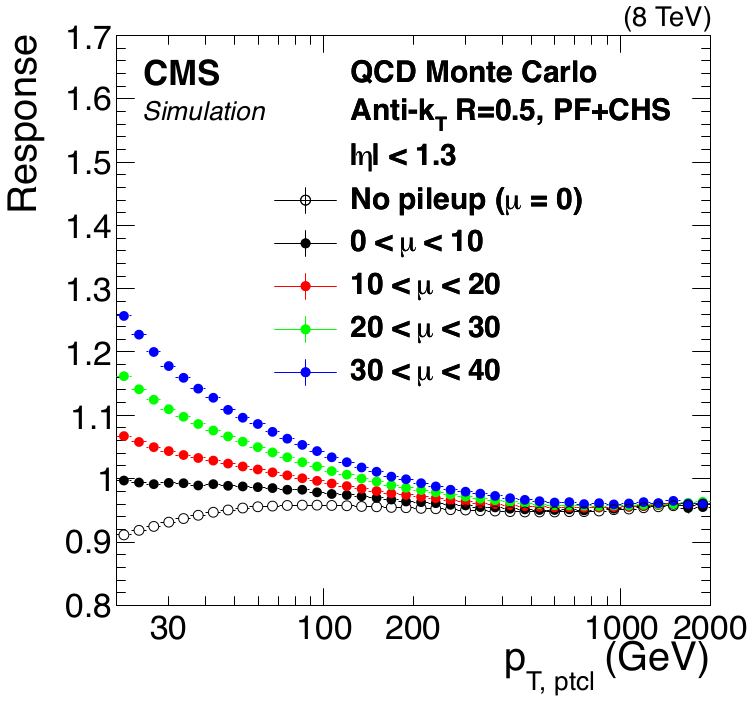
\includegraphics[height = \textheight/2]{\PhDthesisdir/plots_and_images/from_JERC_RunI/response_evolution_1.png}
\hfill
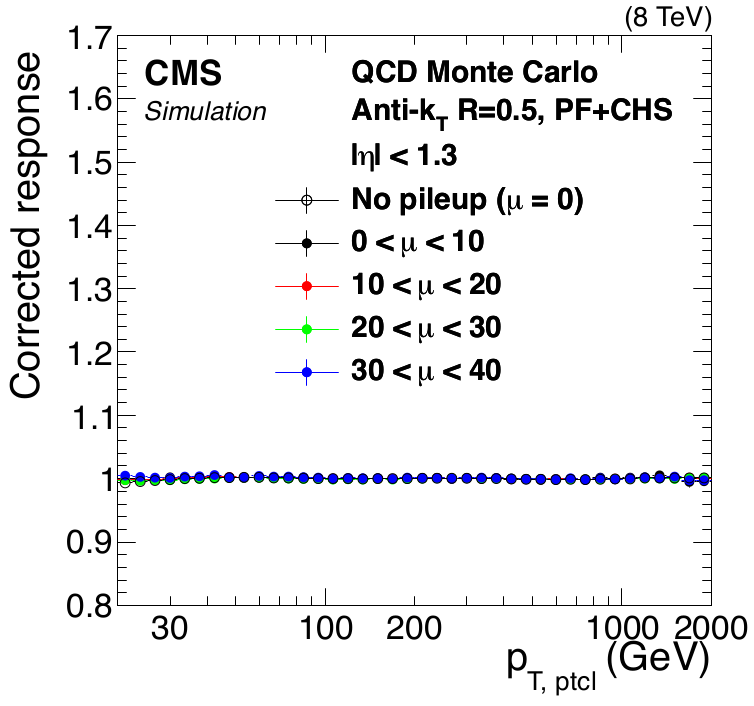
\includegraphics[height = \textheight/2]{\PhDthesisdir/plots_and_images/from_JERC_RunI/response_evolution_3.png}
\end{frame}

\begin{frame}[t]
\addtocounter{framenumber}{-1}
%\transdissolve
\large
\includegraphics[width=\textwidth]{\PhDthesisdir/plots_and_images/from_JERC_RunI/CMS-JME-13-004_Figure_002-FR-TeX-sequential_for_slides/2.tex}

\vfill

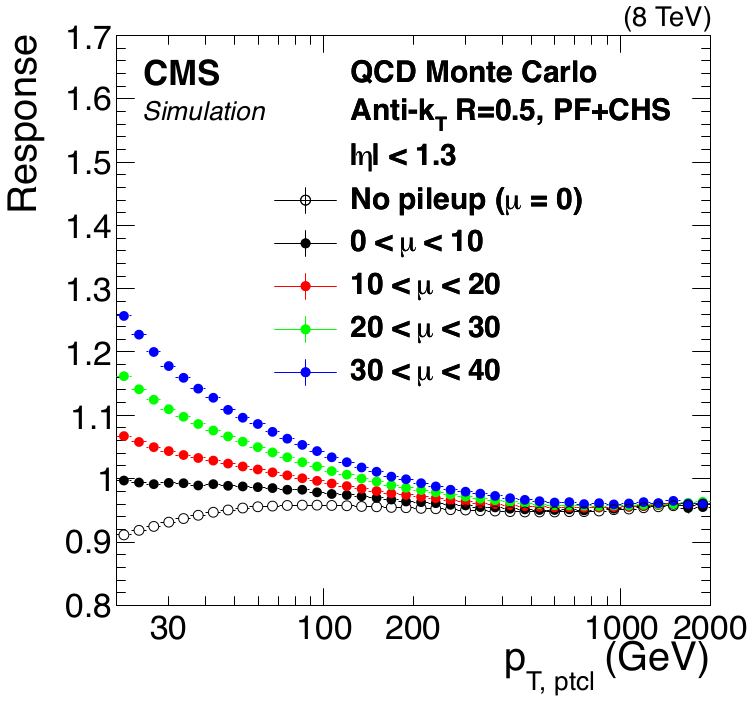
\includegraphics[height = \textheight/2]{\PhDthesisdir/plots_and_images/from_JERC_RunI/response_evolution_1.png}
\hfill
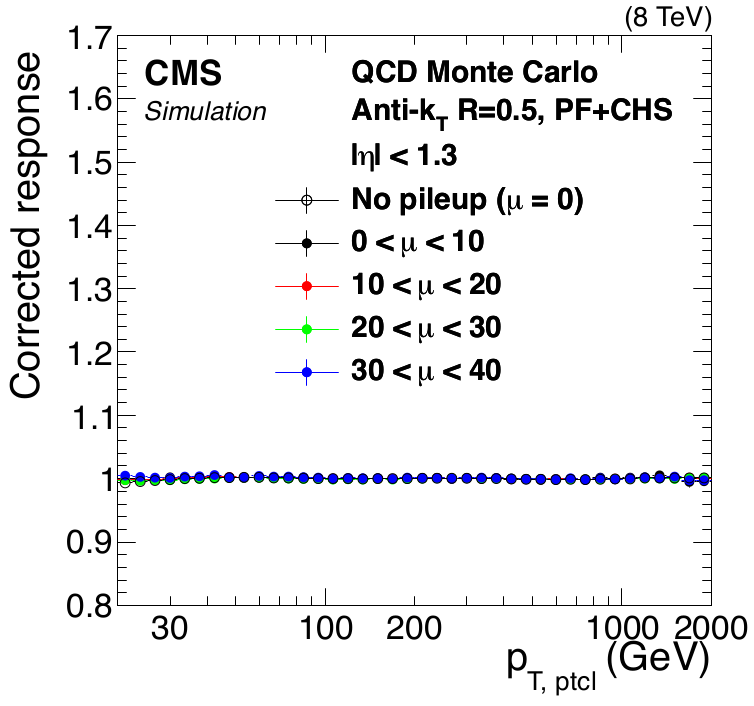
\includegraphics[height = \textheight/2]{\PhDthesisdir/plots_and_images/from_JERC_RunI/response_evolution_3.png}
\end{frame}

\begin{frame}[t]
\addtocounter{framenumber}{-1}
%\transdissolve
\large
\includegraphics[width=\textwidth]{\PhDthesisdir/plots_and_images/from_JERC_RunI/CMS-JME-13-004_Figure_002-FR-TeX-sequential_for_slides/3.tex}

\vfill

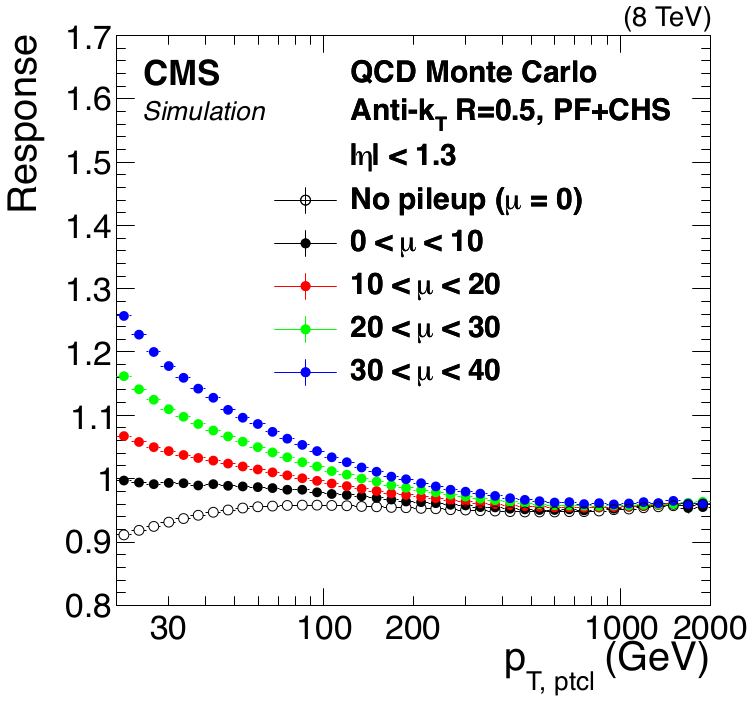
\includegraphics[height = \textheight/2]{\PhDthesisdir/plots_and_images/from_JERC_RunI/response_evolution_1.png}
\hfill
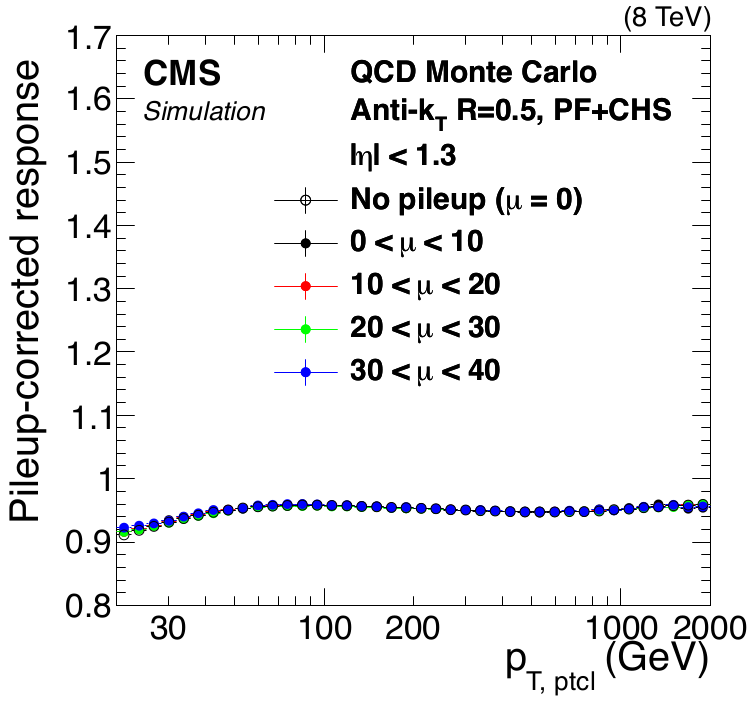
\includegraphics[height = \textheight/2]{\PhDthesisdir/plots_and_images/from_JERC_RunI/response_evolution_2.png}
\hfill
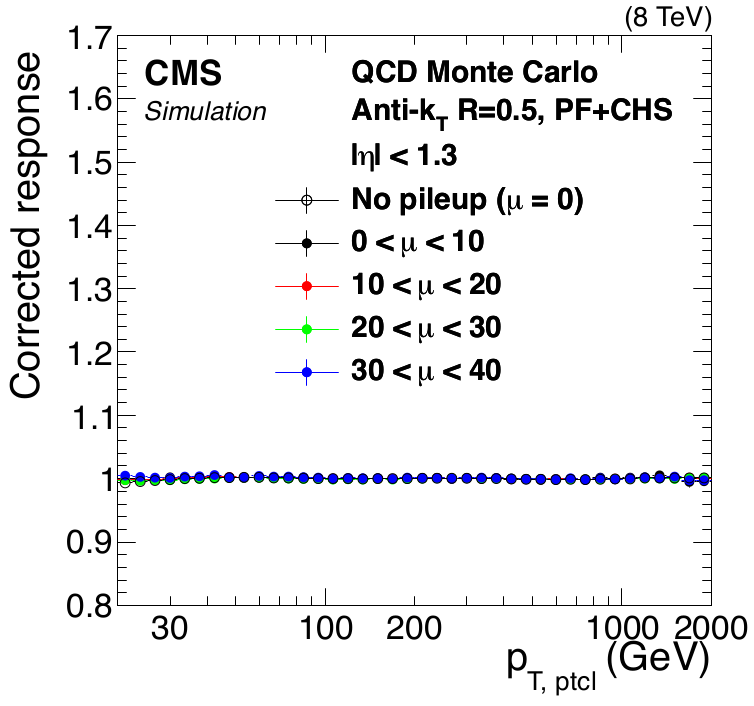
\includegraphics[height = \textheight/2]{\PhDthesisdir/plots_and_images/from_JERC_RunI/response_evolution_3.png}
\end{frame}

\begin{frame}[t]
\addtocounter{framenumber}{-1}
%\transdissolve
\large
\includegraphics[width=\textwidth]{\PhDthesisdir/plots_and_images/from_JERC_RunI/CMS-JME-13-004_Figure_002-FR-TeX-sequential_for_slides/4.tex}

\vfill

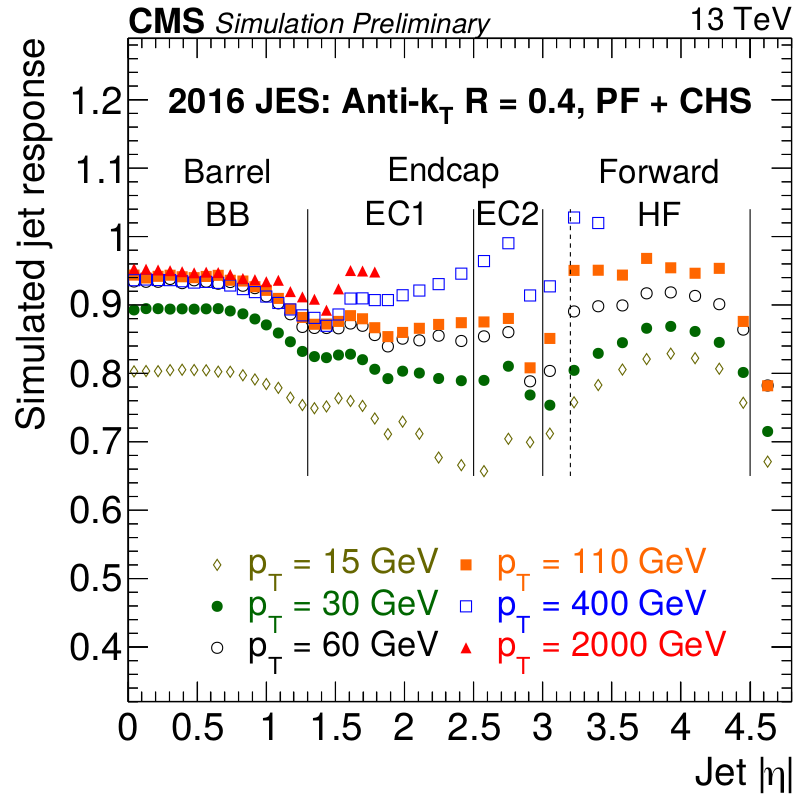
\includegraphics[height = \textheight/2]{\PhDthesisdir/plots_and_images/from_CMS-DP-2020-019/simulated_jet_response_2016.png}
\hfill
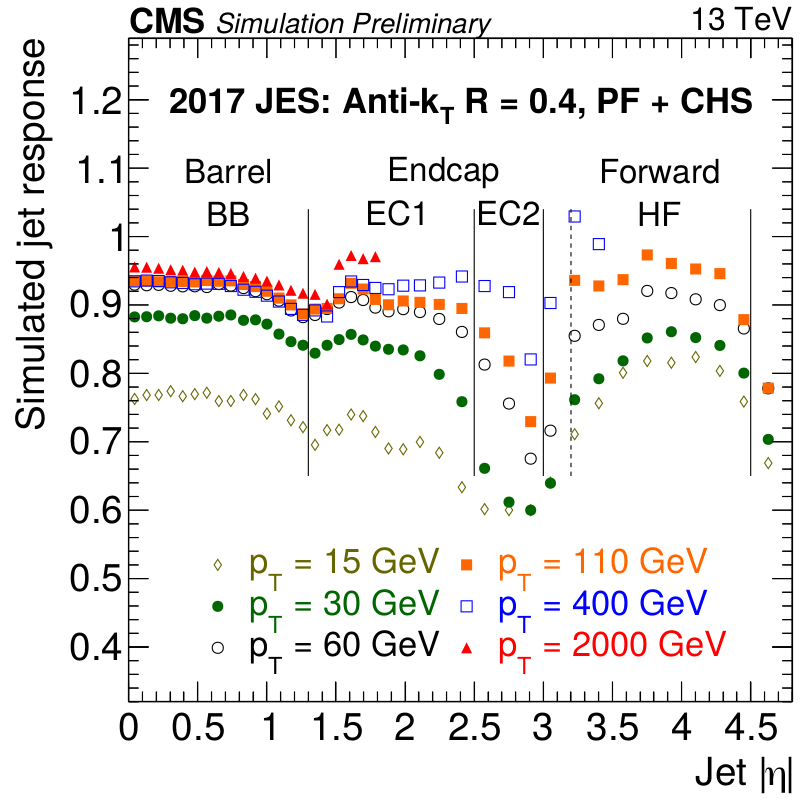
\includegraphics[height = \textheight/2]{\PhDthesisdir/plots_and_images/from_CMS-DP-2020-019/simulated_jet_response_2017.png}
\hfill
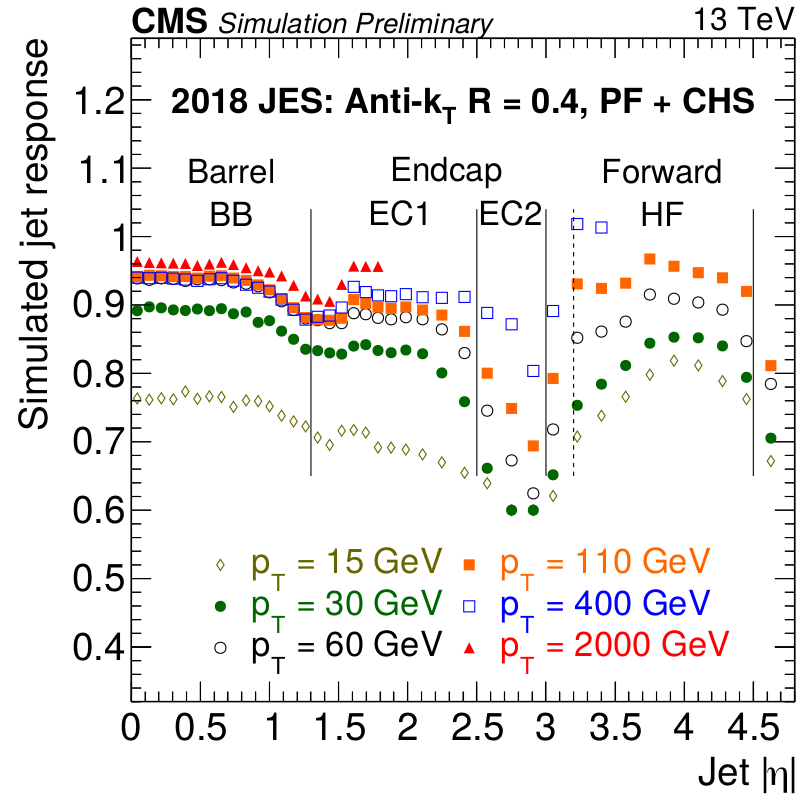
\includegraphics[height = \textheight/2]{\PhDthesisdir/plots_and_images/from_CMS-DP-2020-019/simulated_jet_response_2018.png}
\end{frame}

\begin{frame}[t]
\addtocounter{framenumber}{-1}
%\transdissolve
\large
\includegraphics[width=\textwidth]{\PhDthesisdir/plots_and_images/from_JERC_RunI/CMS-JME-13-004_Figure_002-FR-TeX-sequential_for_slides/5.tex}
\end{frame}

\begin{frame}[t]
\addtocounter{framenumber}{-1}
%\transdissolve
\large
\includegraphics[width=\textwidth]{\PhDthesisdir/plots_and_images/from_JERC_RunI/CMS-JME-13-004_Figure_002-FR-TeX-sequential_for_slides/6.tex}

\vfill

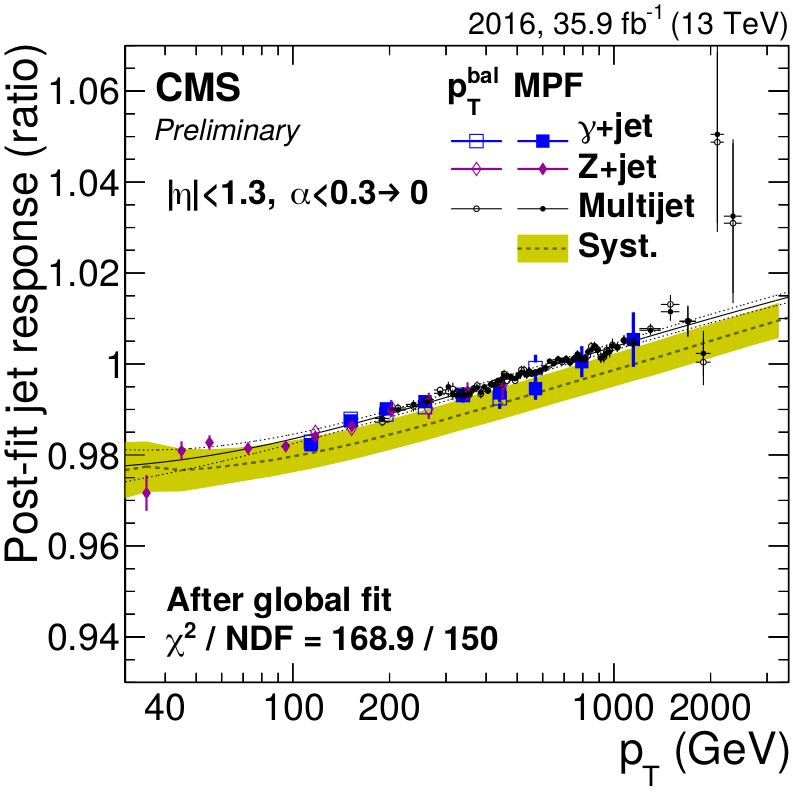
\includegraphics[height = \textheight/2]{\PhDthesisdir/plots_and_images/from_CMS-DP-2020-019/absolute_pT_residual_2016.png}
\hfill
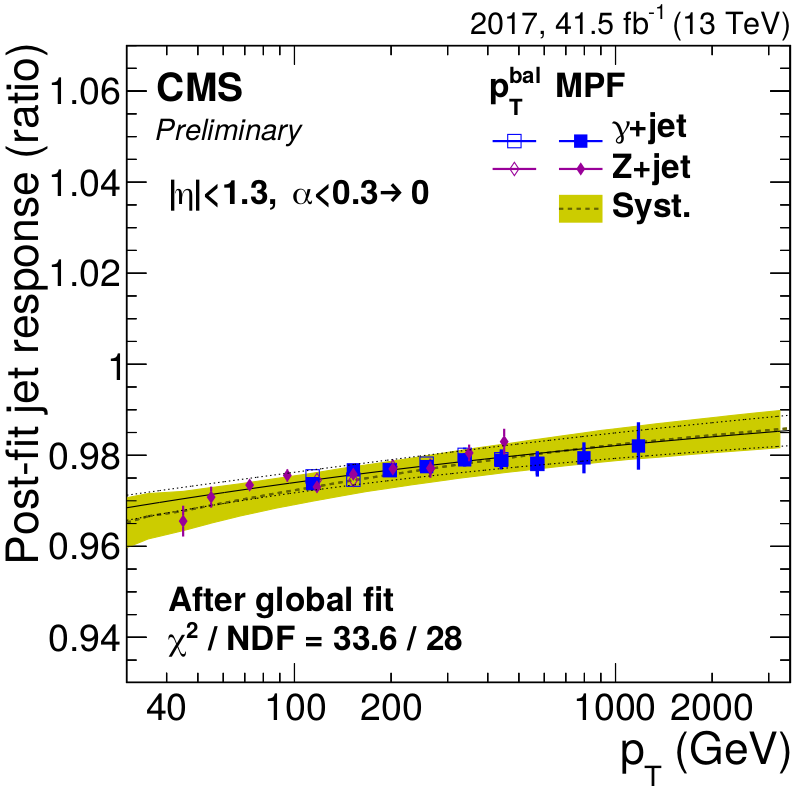
\includegraphics[height = \textheight/2]{\PhDthesisdir/plots_and_images/from_CMS-DP-2020-019/absolute_pT_residual_2017.png}
\hfill
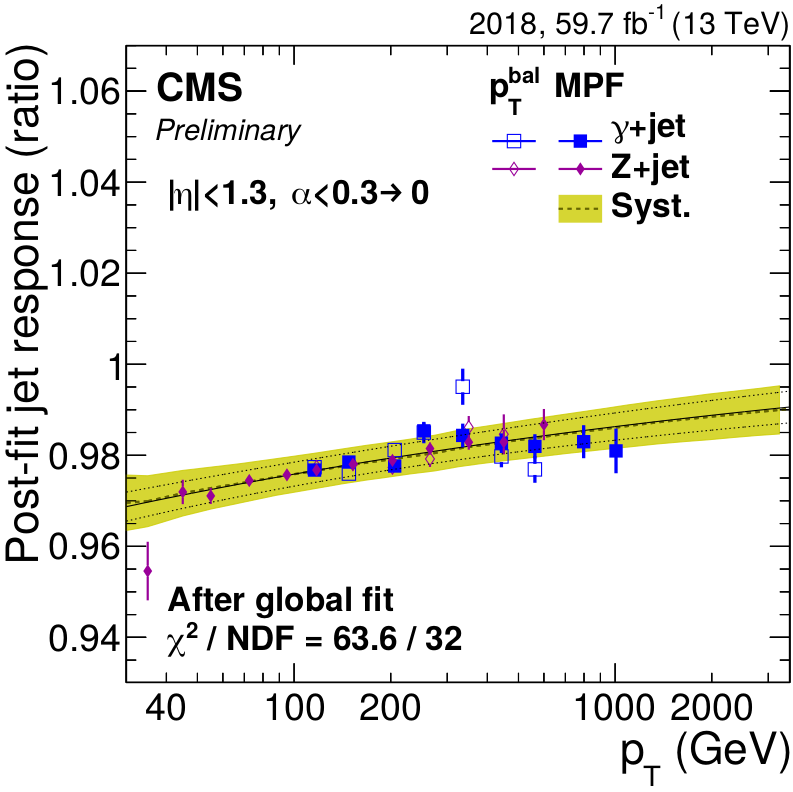
\includegraphics[height = \textheight/2]{\PhDthesisdir/plots_and_images/from_CMS-DP-2020-019/absolute_pT_residual_2018.png}
\end{frame}

\begin{frame}[t]
\addtocounter{framenumber}{-1}
%\transdissolve
\large
\includegraphics[width=\textwidth]{\PhDthesisdir/plots_and_images/from_JERC_RunI/CMS-JME-13-004_Figure_002-FR-TeX.tex}

\vfill

\begin{center}
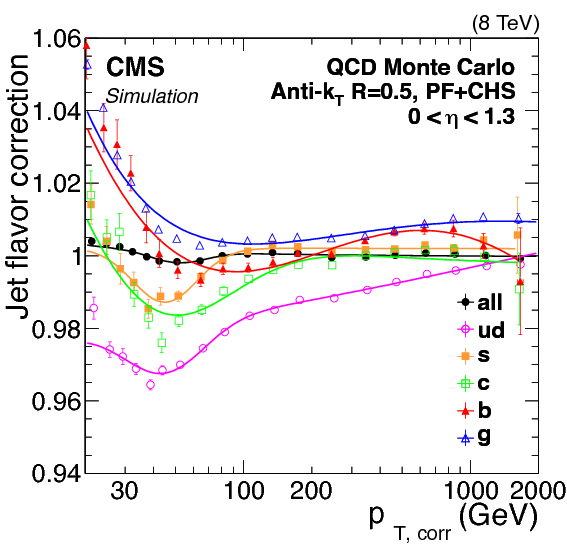
\includegraphics[height = \textheight/2]{\PhDthesisdir/plots_and_images/from_JERC_RunI/Figure_030-a.png}
\end{center}
\end{frame}



%\input{\PhDthesisdir/slides/JERC/JEC_Principe/slides_anims/Gamma_plus_jet.tex}
\begin{frame}
\begin{center}
\includegraphics[width=\graphw,height=\graphh,keepaspectratio]{\PhDthesisdir/plots_and_images/Event_displays/JERC/Gamma_plus_jet.tex}
\end{center}
\end{frame}

\begin{frame}[t]
\vspace{\baselineskip}

~\hfill
\input{\PhDthesisdir/plots_and_images/Feynman_diagrams/Gamma_plus_jets/fgraph-gq_qGamma_S.tex}
\hfill\hfill\hfill
\input{\PhDthesisdir/plots_and_images/Feynman_diagrams/Gamma_plus_jets/fgraph-gq_qGamma_T.tex}
\hfill\hfill\hfill
\input{\PhDthesisdir/plots_and_images/Feynman_diagrams/Gamma_plus_jets/fgraph-qq_gGamma.tex}
\hfill~

\pause
\vfill

\begin{equation*}
\vpT_\ptcl^{\photon} + \vpT_\ptcl^\text{jet} = \vec{0}
\Rightarrow
\pT_\ptcl^{\photon} = \pT_\ptcl^\text{jet}
\end{equation*}
\pause
\begin{equation*}
R
= \frac{\pT_\reco^\text{jet}}{\pT_\ptcl^\text{jet}}
= \frac{\pT_\reco^\text{jet}}{\pT_\ptcl^{\photon}}
\simeq \frac{\pT_\reco^\text{jet}}{\pT_\reco^{\photon}}
\end{equation*}
\pause
\begin{equation*}
\Rbal = \frac{\pT_\reco^\text{jet}}{\pT^{\photon}}
\end{equation*}

%\manip Only 2 \og particles \fg{} (physics objects) in final state:
%\begin{itemize}
%\item photon (well known);
%\item jet (to calibrate).
%\end{itemize}
%\manip No neutrino $\Rightarrow$ no real \MET.
\end{frame}

%\input{\PhDthesisdir/slides/JERC/JEC_Principe/slides_anims/Gamma_plus_2jets.tex}
\begin{frame}
\begin{center}
\includegraphics[width=\graphw,height=\graphh,keepaspectratio]{\PhDthesisdir/plots_and_images/Event_displays/JERC/Gamma_plus_2jets.tex}
\end{center}
\end{frame}

\begin{frame}[t]
\vspace{\baselineskip}

~\hfill
\input{\PhDthesisdir/plots_and_images/Feynman_diagrams/Gamma_plus_jets/fgraph-gq_qGamma_T.tex}
\hfill~

\pause
\vfill

~\hfill
\input{\PhDthesisdir/plots_and_images/Feynman_diagrams/Gamma_plus_jets/fgraph-gq_qGamma_S-ISR_2jets.tex}
\hfill\hfill\hfill
\input{\PhDthesisdir/plots_and_images/Feynman_diagrams/Gamma_plus_jets/fgraph-gq_qGamma_S-ISR_2photons.tex}
\hfill\hfill\hfill
\input{\PhDthesisdir/plots_and_images/Feynman_diagrams/Gamma_plus_jets/fgraph-gq_qGamma_S-FSR_2jets.tex}
\hfill\hfill\hfill
\input{\PhDthesisdir/plots_and_images/Feynman_diagrams/Gamma_plus_jets/fgraph-gq_qGamma_S-FSR_2photons.tex}
\hfill~

\end{frame}

\begin{frame}
\begin{minipage}[t]{.45\textwidth}
\begin{equation*}
\Rbal = \frac{\pT_\reco^\text{jet 1}}{\pT^{\photon}}
\end{equation*}
\end{minipage}
\hfill
\begin{minipage}[t]{.45\textwidth}
\begin{equation*}
\alpha = \frac{\pT_\reco^\text{jet 2}}{\pT^{\photon}}
\end{equation*}
\end{minipage}
\end{frame}

\begin{frame}

\begin{equation*}
\vpT^\photon_\ptcl + \vpT^\text{recul}_\ptcl = \vec{0}
\end{equation*}

\pause
\vfill


\begin{equation*}
\vpT^\photon_\reco + \underbrace{\RMPF \vpT^\text{recul}_\ptcl}_{\vpT^\text{recul}_\reco} = -\vMET
\Rightarrow
\boxed{\RMPF = 1 + \frac{\vpT^\photon\cdot\vMET}{\abs{\vpT^\photon}^2}}
\end{equation*}
\end{frame}
\begin{frame}
\frametitle{$\photon+\text{jet}$ events: jet calibration, balancing method}
\manip The physics of the events gives
\begin{equation*}
\vpT^\photon_\ptcl + \vpT^\text{jet}_\ptcl = \vec{0} \Rightarrow \boxed{{\pT}^\photon_\ptcl = {\pT}^\text{jet}_\ptcl}
\end{equation*}

\pause
\vfill

\manip For the reconstructed objects, the balancing response is then defined as
\begin{equation*}
\vpT^\photon_\reco + \underbrace{\Rbal \vpT^\text{jet}_\ptcl}_{\vpT^\text{jet}_\reco} = \vec{0}
\Rightarrow
\boxed{\Rbal = \frac{{\pT}^\text{jet}_\reco}{\pT^\photon}}
\end{equation*}
\begin{equation*}
\text{because }
\pT^\photon_\ptcl\simeq\pT^\photon_\reco
=\pT^\photon
\mend
\end{equation*}
\end{frame}

\begin{frame}
\frametitle{$\photon+\text{jet}$ events: world is not perfect}
\begin{center}
\includegraphics[width=\graphw,height=\graphh,keepaspectratio, trim = 5.5cm 2cm 7.5cm 1.75cm, clip]{\PhDthesisdir/tex/slides/JERC/JEC_Principe/Gamma_plus_two_jets.pdf}
\end{center}
\end{frame}

\begin{frame}
\frametitle{$\photon+\text{jet}$ events: world is not perfect}
\manip Imbalance due to the presence of additionnal jets.
\pause
\manip Use the jet with higher \pT: $\displaystyle \boxed{\Rbal = \frac{{\pT}^\text{1\up{st}jet}_\reco}{\pT^\photon}}$.
\pause
\manip To avoid correction on additonnal jets: define $\displaystyle \boxed{\alpha = \frac{{\pT}^\text{2\up{nd}jet}_\reco}{\pT^\photon}}$ and extrapolate to $\alpha=0$.
\end{frame}

\begin{frame}
\frametitle{$\photon+\text{jet}$ events: jet calibration, MPF method}
\manip Considering balance between photon and \emph{all other particles},
\begin{equation*}
\vpT^\photon_\ptcl + \vpT^\text{recoil}_\ptcl = \vec{0}
\end{equation*}

\pause
\vfill

\manip For the reconstructed objects, the MPF response is then defined as
\begin{equation*}
\vpT^\photon_\reco + \underbrace{\RMPF \vpT^\text{recoil}_\ptcl}_{\vpT^\text{recoil}_\reco} = -\vMET
\Rightarrow
\boxed{\RMPF = 1 + \frac{\vpT^\photon\cdot\vMET}{\abs{\vpT^\photon}^2}}
\end{equation*}
\end{frame}
\begin{frame}
\frametitle{Run 2018 ABCD responses, $\alpha=\num{0.15}$, $\eta\in [\num{0},\num{1.3}]$}
\begin{minipage}{.45\textwidth}
\begin{figure}
\includegraphics[width=.9\linewidth]{\PhDthesisdir/contents/chapter-JERC/plots/2019-07-25/only_L2Res/Run2018ABCD/alpha_0_15/response_eta0013_balancing.pdf}
\caption{Balancing}
\end{figure}
\end{minipage}
\hfill
\begin{minipage}{.45\textwidth}
\begin{figure}
\includegraphics[width=.9\linewidth]{\PhDthesisdir/contents/chapter-JERC/plots/2019-07-25/only_L2Res/Run2018ABCD/alpha_0_15/response_eta0013_mpf.pdf}
\caption{MPF}
\end{figure}
\end{minipage}
\end{frame}

\begin{frame}
\frametitle{Run 2018 ABCD responses, extrapolation, $\pT\in [\num{175},\num{230}]\SI{}{\GeV}$, $\eta\in [\num{0},\num{1.3}]$}
\begin{minipage}{.45\textwidth}
\begin{figure}
\includegraphics[width=.9\linewidth]{\PhDthesisdir/contents/chapter-JERC/plots/2019-07-25/only_L2Res/Run2018ABCD/extrapolation/response_eta0013_ptPhot_175_230.pdf}
\caption{Balancing}
\end{figure}
\end{minipage}
\hfill
\begin{minipage}{.45\textwidth}
\begin{figure}
\includegraphics[width=.9\linewidth]{\PhDthesisdir/contents/chapter-JERC/plots/2019-07-25/only_L2Res/Run2018ABCD/extrapolation/responseMPF_eta0013_ptPhot_175_230.pdf}
\caption{MPF}
\end{figure}
\end{minipage}
\end{frame}

\begin{frame}
\frametitle{Run 2018 ABCD responses, extrapolated, $\eta\in [\num{0},\num{1.3}]$}
\begin{minipage}{.45\textwidth}
\begin{figure}
\includegraphics[width=.9\linewidth]{\PhDthesisdir/contents/chapter-JERC/plots/2019-07-25/only_L2Res/Run2018ABCD/extrapolated/response_eta0013_balancing_extrap.pdf}
\caption{Balancing}
\end{figure}
\end{minipage}
\hfill
\begin{minipage}{.45\textwidth}
\begin{figure}
\includegraphics[width=.9\linewidth]{\PhDthesisdir/contents/chapter-JERC/plots/2019-07-25/only_L2Res/Run2018ABCD/extrapolated/response_eta0013_mpf_extrap.pdf}
\caption{MPF}
\end{figure}
\end{minipage}
\end{frame}


\begin{frame}
\frametitle{Jet Energy Resolution}
\manip Remember \Rbal\ definition,
\begin{equation*}
\Rbal = \frac{{\pT}^\text{1\up{st}jet}_\text{reco}}{\pT^\photon_\text{reco}}
\end{equation*}

\pause

Then
\begin{equation*}
\Rbal
=
\underbrace{\frac{{\pT}^\text{1\up{st}jet}_\text{reco}}{{\pT}^\text{1\up{st}jet}_\text{ptcl}}}_{\sigma_\text{jet}=\text{JER}}
\times
\underbrace{\frac{{\pT}^\text{1\up{st}jet}_\text{ptcl}}{\pT^\photon_\text{ptcl}}
\vphantom{\frac{{\pT}^\text{1\up{st}jet}_\text{reco}}{{\pT}^\text{1\up{st}jet}_\text{ptcl}}}}_{\text{PLI}}
\times
\underbrace{\frac{\pT^\photon_\text{ptcl}}{\pT^\photon_\text{reco}}
\vphantom{\frac{{\pT}^\text{1\up{st}jet}_\text{reco}}{{\pT}^\text{1\up{st}jet}_\text{ptcl}}}}_{\sigma_\photon\equiv1}
\end{equation*}
\manip PLI: Particle Level Imbalance (pile-up, radiations, neutrinos...), $\to0$ when $\alpha\to0$.

\pause
\begin{equation*}
\boxed{\text{JER} = \sigma_\text{jet} =  \sqrt{\sigma_\Rbal^2 - \sigma_\text{PLI}^2}}
\end{equation*}
\end{frame}


\begin{frame}
\frametitle{Run 2018 ABCD jet resolution}
\begin{minipage}{.45\textwidth}
\begin{figure}
\includegraphics[width=\linewidth]{\PhDthesisdir/plots_and_images/my_plots/JERC/JER/Run2018ABCD/extrapolation/resolution_eta0005_ptPhot_400_500.pdf}
\caption{Extrapolation}
\end{figure}
\end{minipage}
\hfill
\begin{minipage}{.45\textwidth}
\begin{figure}
\includegraphics[width=\linewidth]{\PhDthesisdir/plots_and_images/my_plots/JERC/JER/Run2018ABCD/alpha_0_3/fine_eta_binning_Scale_factor_res_vs_ETA.pdf}
\caption{Scale factor}
\end{figure}
\end{minipage}
\end{frame}

\begin{frame}\addtocounter{framenumber}{-1}
\frametitle{Run 2018 ABCD jet resolution}
\begin{minipage}{.45\textwidth}
\begin{figure}
\includegraphics[width=\linewidth, trim=0cm 0cm 3cm 0cm]{\PhDthesisdir/plots_and_images/from_CMS_alignment_photodetectors/CMS-eta-ranges.png}
\caption{CMS and $\eta$ values}
\end{figure}
\end{minipage}
\hfill
\begin{minipage}{.45\textwidth}
\begin{figure}
\includegraphics[width=\linewidth]{\PhDthesisdir/plots_and_images/my_plots/JERC/JER/Run2018ABCD/alpha_0_3/fine_eta_binning_Scale_factor_res_vs_ETA.pdf}
\caption{Scale factor}
\end{figure}
\end{minipage}
\end{frame}



\subsection*{Triggers efficiencies}
\begin{frame}
\backupslinklabel{trgeffs}
\frametitle{Triggers in the \tauh\tauh\ channel}

\begin{minipage}[c]{.45\textwidth}
\manip In the manuscript: page 118, formula (4.5)
\begin{align*}
\epsilon &=
{\color{ltcolorblue}\epsilon(2\tauh) + \epsilon(\tauh1) + \epsilon(\tauh2)}
\nonumber\\ & \hphantom{=}
{\color{ltcolorgreen}- \epsilon(2\tauh + \tauh1) - \epsilon(2\tauh + \tauh1) - \epsilon(\tauh1+\tauh2)}
\nonumber\\ & \hphantom{=}
{\color{ltcolorred}+ \epsilon(2\tauh + \tauh1 + \tauh2)}
\end{align*}
\end{minipage}
\hfill
\begin{minipage}[c]{.45\textwidth}
\begin{center}
\begin{tikzpicture}
\def\rcircle{1.5}
\def\overlappct{.6}

\fill [ltcolorblue2] (-90:\overlappct*\rcircle) circle (\rcircle);
\fill [ltcolorblue2] (-90+120:\overlappct*\rcircle) circle (\rcircle);
\fill [ltcolorblue2] (-90-120:\overlappct*\rcircle) circle (\rcircle);

\begin{scope}
\clip (-90:\overlappct*\rcircle) circle (\rcircle);
\clip (-90-120:\overlappct*\rcircle) circle (\rcircle);
\fill [ltcolorgreen2] (-90:\overlappct*\rcircle) circle (\rcircle);
\end{scope}

\begin{scope}
\clip (-90:\overlappct*\rcircle) circle (\rcircle);
\clip (-90+120:\overlappct*\rcircle) circle (\rcircle);
\fill [ltcolorgreen2] (-90:\overlappct*\rcircle) circle (\rcircle);
\end{scope}

\begin{scope}
\clip (-90+120:\overlappct*\rcircle) circle (\rcircle);
\clip (-90-120:\overlappct*\rcircle) circle (\rcircle);
\fill [ltcolorgreen2] (-90+120:\overlappct*\rcircle) circle (\rcircle);
\end{scope}

\begin{scope}
\clip (-90:\overlappct*\rcircle) circle (\rcircle);
\clip (-90+120:\overlappct*\rcircle) circle (\rcircle);
\clip (-90-120:\overlappct*\rcircle) circle (\rcircle);
\fill [ltcolorred2] (-90+120:\overlappct*\rcircle) circle (\rcircle);
\end{scope}

\draw (-90:\overlappct*\rcircle) circle (\rcircle);
\draw (-90+120:\overlappct*\rcircle) circle (\rcircle);
\draw (-90-120:\overlappct*\rcircle) circle (\rcircle);

\draw (-90:\overlappct*\rcircle+.5*\rcircle) node {2\tauh} ;
\draw (-90+120:\overlappct*\rcircle+.5*\rcircle) node {\tauh2} ;
\draw (-90-120:\overlappct*\rcircle+.5*\rcircle) node {\tau1} ;

\end{tikzpicture}
\end{center}
\end{minipage}

\end{frame}

\subsection*{Subleading \ftauh}
\begin{frame}
\backupslinklabel{subleadingFtauh}
\frametitle{\Fakefactors\ for subleading \tauh}

\manip The \tauh\tauh\ \fakefactors\ are measured for the leading \tauh\ candidate only.
\submanip The subleading one can be either a genuine or fake \tauh.

\manip At this point, underestimation of events in which only the subleading \tauh\ is a fake.
\submanip Adding these back using MC.

\manip Small fraction of fakes $<\SI{10}{\%}$ in \CATnobtag, $<\SI{30}{\%}$ in \CATbtag\ (due to \ttbar):

~\hfill
\includegraphics[width=.35\textwidth]{/home/torterotot/Documents/PhD-Thesis/plots_and_images/from_CMS-NOTE-2020-218/wFakes_over_jetFakes_nobtag.pdf}
\hfill
\includegraphics[width=.35\textwidth]{/home/torterotot/Documents/PhD-Thesis/plots_and_images/from_CMS-NOTE-2020-218/wFakes_over_jetFakes_btag.pdf}
\hfill~

\vspace{-5pt}

\beamercite{CMS-NOTE-2020-218}

\begin{tikzpicture}[overlay, remember picture]
\draw (.2\textwidth, .35\textheight) node {\CATnobtag};
\draw (.7\textwidth, .35\textheight) node {\CATbtag};
\end{tikzpicture}
\end{frame}

\subsection*{Custom loss function}
\begin{frame}
\backupslinklabel{custom_loss}
%\frametitle{Custom loss function for the DNN -- mass range effect}

\begin{minipage}[c]{.475\textwidth}
\only<1>{\begin{center}\vspace{-4pt}
\begin{tikzpicture}%
\node[anchor=south west,inner sep=0] at (0,0) {\includegraphics[height=\graphh]{\PhDthesisdir/plots_and_images/my_plots/ML/from_ML_plots/DNNs_for_discussion/Mass_range/predicted_vs_answers_histo-NN-activation-softplus-batch_size-2048-mape-Adam-gu-inclusive-3-layers-1000-neurons-en.pdf}};

\draw [ltcolororange, thick] (2.45, 1.1) -- (2.45, 6.7);
\draw [ltcolororange, thick] (3.985, 1.1) -- (3.985, 6.7);

\draw [ltcolorviolet, thick] (1.5, 2.2) -- (6.5, 2.2);
\draw [ltcolorviolet, thick] (1.5, 3.9) -- (6.5, 3.9);

\end{tikzpicture}
\end{center}}
\only<2>{
\manip {\color{ltcolorred} How to cope with the boundaries?}
\submanip Bias to be balanced,
\submanip Extend the mass range?
\subsubmanip Would be nice!
\subsubmanip Not always feasible...

\manip Every horizontal slice is one predicted value:
\submanip \og Same family \fg{} of events to the NN.
%\submanip Actually $\sim$ centered on the red line!
%\subsubmanip {\footnotesize Center of the distributions in the red rectangles.}
}

\only<3>{\begin{center}\vspace{-4pt}
\begin{tikzpicture}%
\node[anchor=south west,inner sep=0] at (0,0) {\includegraphics[height=\graphh]{\PhDthesisdir/plots_and_images/my_plots/ML/from_ML_plots/DNNs_for_discussion/Mass_range/distributions/distribution-inclusive-Higgs_mass_gen-at_pred_mass_400weighted-is_test-en.pdf}};

\draw (6.5, 6) node [left] {\small $\sim$ Symmetric \OK};
\end{tikzpicture}
\end{center}}
\only<4>{\begin{center}\vspace{-4pt}
\begin{tikzpicture}%
\node[anchor=south west,inner sep=0] at (0,0) {\includegraphics[height=\graphh]{\PhDthesisdir/plots_and_images/my_plots/ML/from_ML_plots/DNNs_for_discussion/Mass_range/distributions/distribution-inclusive-Higgs_mass_gen-at_pred_mass_750weighted-is_test-en.pdf}};

\draw (1.5, 6) node [right] {\small Cropped distribution!};
\draw (1.5, 5.25) node [right] {\small Only low mass tail is here:};
\draw (1.5, 4.25) node [right, text width=3.5cm] {\scriptsize With full distribution, the DNN would have learnt to predict higher values};
\end{tikzpicture}
\end{center}}
\end{minipage}
\hfill
\begin{minipage}[c]{.475\textwidth}
\begin{center}\vspace{-4pt}
\begin{tikzpicture}
\node[anchor=south west,inner sep=0] at (0,0) {\includegraphics[height=\graphh]{\PhDthesisdir/plots_and_images/my_plots/ML/from_ML_plots/trained_NNs_FastSim/DeepTau-inclusive/PuppiMET_with_METcov_j1j2jr_Nnu_Npu/predicted_vs_answers_histo-NN-ADAM_glorot_uniform-activation-softplus-batch_size-2048-mape-Adadelta-u-inclusive-3-layers-1000-neurons-en.pdf}};

\only<1>{
\draw [ltcolororange, thick] (1.675, 1.1) -- (1.675, 6.7);
\draw [ltcolororange, thick] (5.55, 1.1) -- (5.55, 6.7);

\draw [ltcolorviolet, thick] (1.5, 1.3) -- (6.5, 1.3);
\draw [ltcolorviolet, thick] (1.5, 5.65) -- (6.5, 5.65);
}

\only<3>{
\draw [ltcolorred, thick] (1.5, 3.25) rectangle (5.55, 3.4);
\draw (2.25, 1.5) node [right] {\small Events at \SI{400}{\GeV} to the NN};
\draw [-latex, ltcolorgreen, thick] (4.25, 1.7) to[in=-45, out=60] (3.75, 3.2);
}

\only<4>{
\draw [ltcolorred, thick] (1.5, 5.25) rectangle (5.55, 5.4);
\draw (2, 6.3) node [right] {\small Events at \SI{750}{\GeV} to the NN};
\draw [-latex, ltcolorgreen, thick] (2.6, 6.1) to[in=135, out=-120] (3, 5.5);
}

\end{tikzpicture}
\end{center}\vspace{-5pt}
\end{minipage}

\end{frame}

\begin{frame}
\begin{minipage}[c]{.475\textwidth}
\begin{center}\vspace{-4pt}
\begin{tikzpicture}%
\node[anchor=south west,inner sep=0] at (0,0) {\includegraphics[height=\graphh]{\PhDthesisdir/plots_and_images/my_plots/ML/from_ML_plots/DNNs_for_discussion/Mass_range/distributions/distribution-inclusive-Higgs_mass_gen-mirrored_cut_at_pred_mass_750weighted-is_test-en.pdf}};

\draw (1.5, 6) node [right] {\small Crop again, restore symmetry};
\end{tikzpicture}
\end{center}
\end{minipage}
\hfill
\begin{minipage}[c]{.475\textwidth}
\begin{center}\vspace{-4pt}
\includegraphics[height=\graphh]{\PhDthesisdir/plots_and_images/my_plots/ML/custom_loss-illustrations/distance_and_mirror-en.tex}
\end{center}\vspace{-5pt}
\end{minipage}
\end{frame}


\begin{frame}

\begin{minipage}[c]{.51\textwidth}
\begin{align*}
\LossMAPEsqrtb(\ytrue, \ypred)
&=
\LossMAPEsqrt(\ytrue, \ypred)
\\&
\times
\left\lbrace
\begin{aligned}
0 \quad & \text{if $(\ytrue, \ypred)\in$ area 3}\\
\num{0.1} \quad & \text{if $(\ytrue, \ypred)\in$ area 4}\\
1 \quad & \text{else}
\end{aligned}
\right.
\end{align*}
\begin{align*}
\LossMAPEsqrt(\ytrue, \ypred)
&=
\LossMAPE(\ytrue, \ypred) \times \sqrt{\ytrue}
\\&=
\abs{\frac{\ypred-\ytrue}{\ytrue}} \times \sqrt{\ytrue}
\nonumber\\\Leftrightarrow
\LossMAPEsqrt(\ytrue, \ypred)
&=
\abs{\frac{\ypred-\ytrue}{\sqrt{\ytrue}}}
\mend
\end{align*}
\end{minipage}
\hfill
\begin{minipage}[c]{.475\textwidth}
\begin{center}\vspace{-4pt}
\includegraphics[height=\graphh]{\PhDthesisdir/plots_and_images/my_plots/ML/custom_loss-illustrations/areas-EN.tex}
\end{center}\vspace{-5pt}
\end{minipage}

\end{frame}